\begin{figure}[ht]
\centering
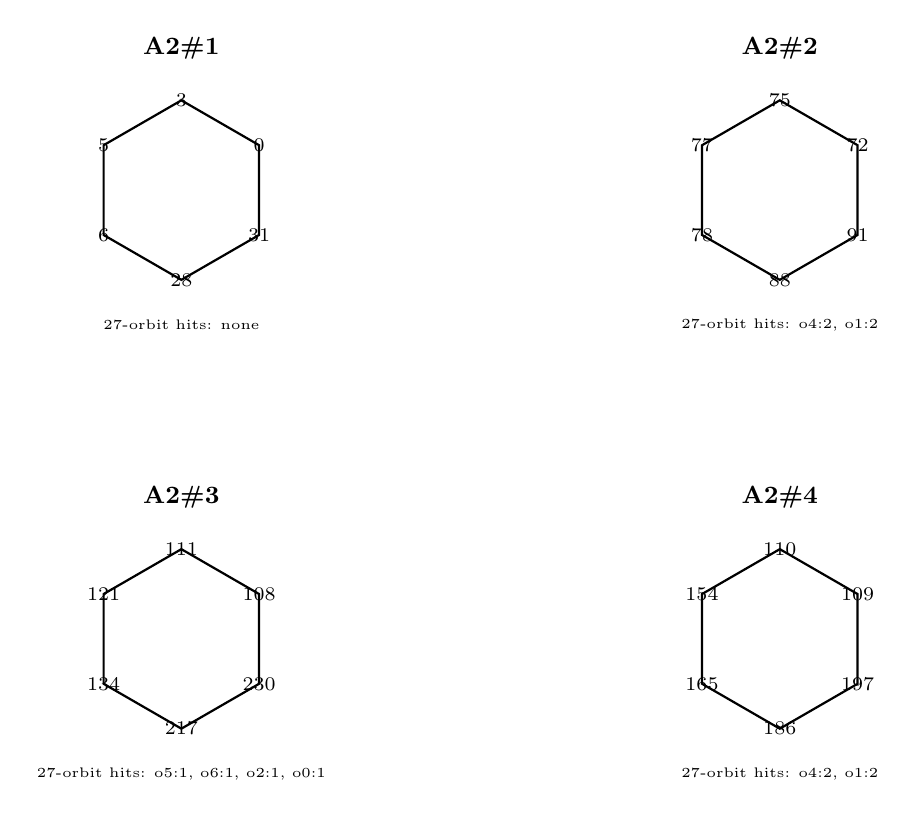
\begin{tikzpicture}[scale=0.95]
\draw[thick] (-2.9607695154586735, 3.5999999999999996) -- (-4.0, 4.2) -- (-5.039230484541326, 3.6000000000000005) -- (-5.039230484541326, 2.4000000000000004) -- (-4.0, 1.8) -- (-2.960769515458674, 2.3999999999999995) -- cycle;
\node[font=\scriptsize] at (-2.96,3.60) {0};
\node[font=\scriptsize] at (-4.00,4.20) {3};
\node[font=\scriptsize] at (-5.04,3.60) {5};
\node[font=\scriptsize] at (-5.04,2.40) {6};
\node[font=\scriptsize] at (-4.00,1.80) {28};
\node[font=\scriptsize] at (-2.96,2.40) {31};
\node[font=\small\bfseries] at (-4.00,4.90) {A2\#1};
\node[font=\tiny] at (-4.00,1.20) {27-orbit hits: none};
\draw[thick] (5.039230484541326, 3.5999999999999996) -- (4.0, 4.2) -- (2.960769515458674, 3.6000000000000005) -- (2.9607695154586735, 2.4000000000000004) -- (4.0, 1.8) -- (5.039230484541326, 2.3999999999999995) -- cycle;
\node[font=\scriptsize] at (5.04,3.60) {72};
\node[font=\scriptsize] at (4.00,4.20) {75};
\node[font=\scriptsize] at (2.96,3.60) {77};
\node[font=\scriptsize] at (2.96,2.40) {78};
\node[font=\scriptsize] at (4.00,1.80) {88};
\node[font=\scriptsize] at (5.04,2.40) {91};
\node[font=\small\bfseries] at (4.00,4.90) {A2\#2};
\node[font=\tiny] at (4.00,1.20) {27-orbit hits: o4:2, o1:2};
\draw[thick] (-2.9607695154586735, -2.4000000000000004) -- (-4.0, -1.8) -- (-5.039230484541326, -2.3999999999999995) -- (-5.039230484541326, -3.5999999999999996) -- (-4.0, -4.2) -- (-2.960769515458674, -3.6000000000000005) -- cycle;
\node[font=\scriptsize] at (-2.96,-2.40) {108};
\node[font=\scriptsize] at (-4.00,-1.80) {111};
\node[font=\scriptsize] at (-5.04,-2.40) {121};
\node[font=\scriptsize] at (-5.04,-3.60) {134};
\node[font=\scriptsize] at (-4.00,-4.20) {217};
\node[font=\scriptsize] at (-2.96,-3.60) {230};
\node[font=\small\bfseries] at (-4.00,-1.10) {A2\#3};
\node[font=\tiny] at (-4.00,-4.80) {27-orbit hits: o5:1, o6:1, o2:1, o0:1};
\draw[thick] (5.039230484541326, -2.4000000000000004) -- (4.0, -1.8) -- (2.960769515458674, -2.3999999999999995) -- (2.9607695154586735, -3.5999999999999996) -- (4.0, -4.2) -- (5.039230484541326, -3.6000000000000005) -- cycle;
\node[font=\scriptsize] at (5.04,-2.40) {109};
\node[font=\scriptsize] at (4.00,-1.80) {110};
\node[font=\scriptsize] at (2.96,-2.40) {154};
\node[font=\scriptsize] at (2.96,-3.60) {165};
\node[font=\scriptsize] at (4.00,-4.20) {186};
\node[font=\scriptsize] at (5.04,-3.60) {197};
\node[font=\small\bfseries] at (4.00,-1.10) {A2\#4};
\node[font=\tiny] at (4.00,-4.80) {27-orbit hits: o4:2, o1:2};
\end{tikzpicture}
\caption{A2$^4$ layer inside E8 (one explicit orthogonal 4-tuple). Numbers are E8 root indices in the standard ordering. The A2 hexagons are global: their roots split across multiple 27-orbits.}
\end{figure}
